\input format

\usepackage{tikz}
\usepackage{graphicx}
\usepackage{amssymb}
\usepackage{amsmath}
\usepackage{harpoon}
\usepackage{float}
\usepackage{enumerate}
\usepackage{algorithm}
\usepackage{algpseudocode}
\usepackage{subcaption}
\usepackage{bm}
\usepackage{listings}

\usetikzlibrary{fit,positioning}

\begin{document}
\begin{flushleft}

\bf{DD2424 Assignment 2 Report (For Basic Part)} \\
\bf{Zesen Wang} \\



\end{flushleft}


\section{Analytic Gradient Computations}
I wrote a function to compute the gradient numerically based on the centered difference formula. Then I use the first 10 data points and the first 400 dimensions as the data for gradient computing. The mean relative differents for $b$ as $W$ are shown below. 

\[
\begin{aligned}
	\text{When }\lambda=0.1,\,\,\,e_{W}=1.1353\cdot 10^{-6},\,\,\,e_{b}=3.2248\cdot 10^{-6}\\
	\text{When }\lambda=0.0,\,\,\,e_{W}=9.2920\cdot 10^{-7},\,\,\,e_{b}=3.2249\cdot 10^{-6}
\end{aligned}
\]

According to the result, the relative difference is acceptable (around $10^{-6}$), which means the analytic gradient computations are correct.

\section{Effect of Momentum}
I train the network with $\texttt{eta=0.01}$, $\texttt{n\_epochs=10}$, $\texttt{lambda=1e-6}$, $\texttt{decay\_rate=0.95}$, $\texttt{n\_batch=100}$, and the $\texttt{momentem (rho)}$ is tested in $\{0, 0.5, 0.9, 0.95, 0.99\}$. The result of the experiments is shown below.

\begin{figure}[h!]
	\centering
	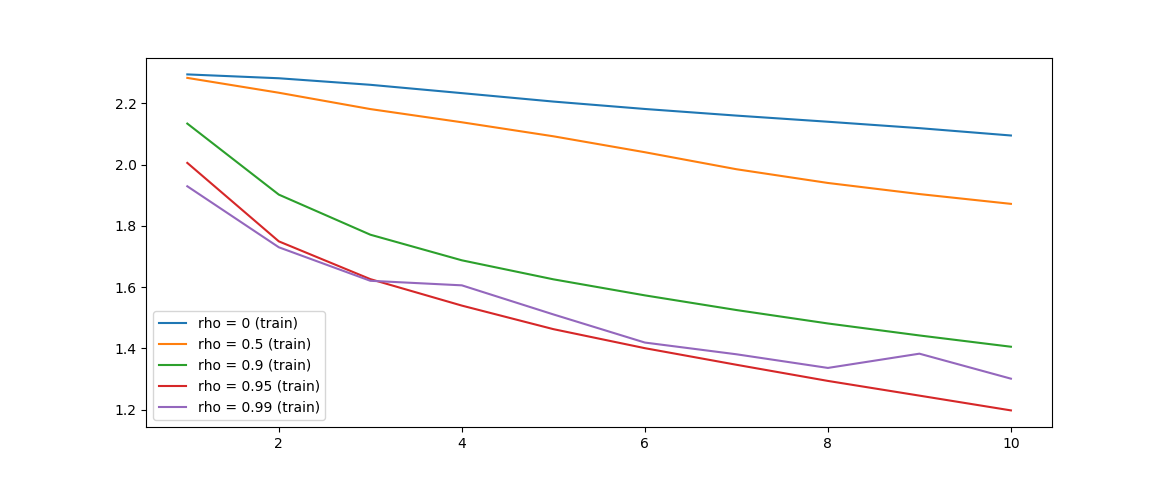
\includegraphics[width=0.9\textwidth]{../Result_imgs/bestrho.png}
\end{figure}

The results show that when $\texttt{rho=0.95}$, the training is boosted most because under same number of epochs, the train loss with momentum is less than the train loss without momentum. And whatever \texttt{rho} is applied, the training process is accelerated, which shows the positive effect of momentum.

\section{Find \texttt{lambda} and \texttt{eta}}

The range I searched for \texttt{lambda} and \texttt{eta} are $[10^{-6}, 10^{-2}]$ and $[10^{-3}, 0.04]$ respectively. I set the \texttt{n\_epoch} as 10, and I calculate the accuracy on validation set for each hyper-parameter setting.

And the three best hyper-parameter settings are

\begin{verbatim}
Accuracy: 0.4472, lambda: 0.0023292248102687557, eta: 0.017453577972249945
Accuracy: 0.4437, lambda: 0.00590089433327251, eta: 0.013611753934771816
Accuracy: 0.4429, lambda: 0.0014195906437909028, eta: 0.018820783416993257
\end{verbatim} 

\section{Train the Network}

The hyperparameter setting is 
\begin{verbatim}
lambda=0.0023292248102687557, eta=0.017453577972249945, 
momemtum=0.95, weight_decay=0.95, n_batch=100, n_epoch=30
\end{verbatim}

\begin{figure}[h!]
	\centering
	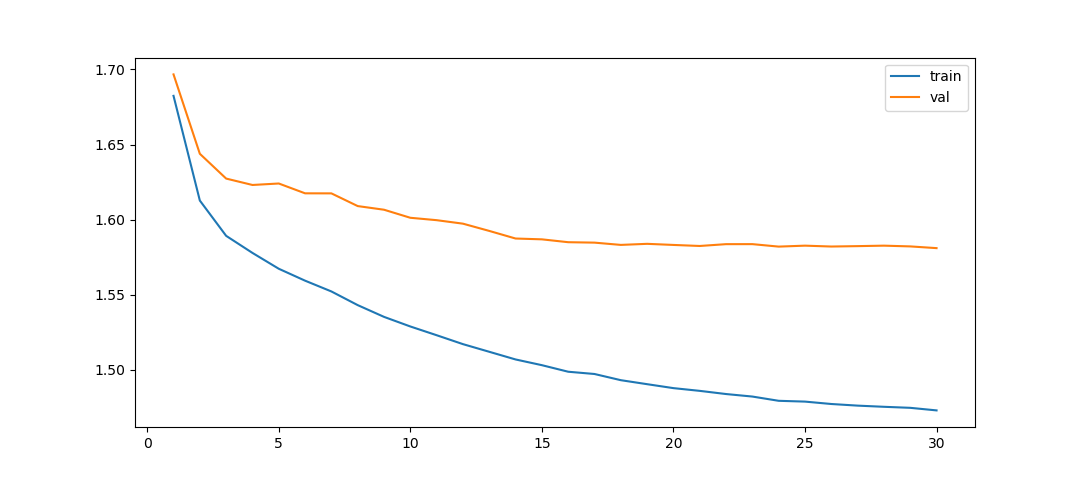
\includegraphics[width=0.9\textwidth]{../Result_imgs/origin.png}
\end{figure}

The accuracy on test set is 0.5127 after 30 epochs.

\end{document}


